\documentclass[12pt]{article}
\setlength {\marginparwidth }{2cm}
\usepackage{amsmath}
\usepackage[margin=1 in]{geometry}
\usepackage{graphicx}
\usepackage{booktabs}
\usepackage{natbib}
\usepackage{lipsum}
\usepackage[colorlinks=true, citecolor=blue]{hyperref}
\usepackage{tabularx}
\usepackage{langsci-optional}
\usepackage{langsci-gb4e}
\usepackage[T1]{fontenc}

\title{The Effect of the COVID-19 Pandemic on Influenza Vaccination Rates in the United States}
\author{Jessica Zambuto\\
Department of Statistics, University of Connecticut}

\begin{document}
\maketitle
\section*{Abstract}
\label{sec:Abstract}
Past research has shown that the influenza vaccination has decreased the likelihood of hospitalization within patients
that test positive for COVID-19 \citep{conlon2021impact}. Thus, maintaning high influenza vaccination rates is essential \
to decreasing the severity of COVID-19 cases. The goal of this study is to determine how influenza vaccination rates within the
United States have changed due to the pandemic by comparing proportions of those vaccinated before the pandemic, defined as 2018-2019
to those during the pandemic, defined as 2020-2021, and comparing during the pandemic to proportions after the pandemic defined as 2021-2022. 
In order to account for possible factors that influence influenza vaccination coverage, the analysis was performed on three groups: by age,
race, and the general population. Results showed that there is statistically significant evidence in favor of a difference in proportions before,
and after the COVID-19 pandemic for the various age groups and the general population. There is no statistically significant evidence of a difference
in proporitions for the racial groups.

\section*{Keywords}
\label{sec:Keywords}
Influenza Vaccine, Statistics, Two Proportion Z-Test, Vaccine Hesitancy

\section{Introduction}
\label{sec:Introduction}
As stated above, studies have indicated that there is an association with influenza vaccinations and improved clinical outcomes. In one retrospective cohort study, clinical outcomes of those who tested
positive for Covid-19 were compared amongst those with and without the influenza vaccine. Clinical outcomes included need for hospitilization, length of stay, need for intensive care, need for ventiliation,
and mortality. The association between influenza vaccination and clinical outcomes were calculated using weighted logistic regression models and a weighted Cox proportional hazards model was used to evalulate
mortality differences among those vaccinated and unvaccinated. Results showed that there was a significant reduction in the odds of testing positive for Covid-19 in patients who recieved the influenza vaccine
(odds ratio .76, 95\% confidence interval .68-.86, p-value <.001); those vaccinated were less likely to require hopsitalization (odds ratio .58, 95\% confidence interval .46-.73, p-value <.001), and required a
shorter hopsital length of stay (odds ratio .76, 95\% confidence interval .65-.89, p-value <.001) \citep{conlon2021impact}. \par
Other studies have indicated that the Covid-19 pandemic has changed influenza vaccination attitudes. For instance, in one retrospective study conducted among Italian cancer healthcare workers during the pandemic, the McNenar's non-parametric
test was conducted to compare vaccination adherence change and a multinomial logistic rgression analysis was performed to assess the relationship between influenza vaccination behaviors and charactertics such as age and gender. Results indicated
that the Covid-19 pandemic inreased adherence to the influenza vaccine amongst these healthcare workers during 2020-2021, but also had an increase in vaccination proportions. This suggested that the pandemic might have been an incentive to get vaccinated
\citep{bertoni2022has}. \par
Similarily, in another Italian cross-sectional study, the beliefs, attitudes, and practices of a representative sample of Italian adults regarding the influenza vaccine was assessed. This was accomplished by calculating adjusted odds ratios between
between not being willing to receive the next seasons influenza vaccination and socioeconomic characteristics using multivariable logistic regression. "to verify the influence of the COVID-19 pandemic on intention to be vaccinated in the 2020/21 season, 
as compared with the previous 2019/20 vaccination, an ordinal logistic regression analysis was performed with the output expressed as the adjusted proportional odds ratio (pOR)" \citep{domnich2020attitudes}. Results showed "most (74.8\%) participants valued 
influenza vaccination positively and declared that it should be mandatory, some misconceptions around influenza persist. Younger and less affluent individuals, subjects not vaccinated in the previous season, and those living in smaller communities showed lower 
odds of receiving the 2020/21 season influenza vaccination. However, the COVID-19 pandemic may have positively influenced the propensity of being vaccinated against 2020/21 seasonal influenza" \citep{domnich2020attitudes}. This study suggested that there could have 
been a difference in proportions of those who recieved the influenza vaccine amongst different age groups. \par
But why have studies shown a difference in influenza vaccination rates during the Covid-19 pandemic?  One study suggested that the pandemic could be considered an incentive that significantly and dramatically increased adherence to flu vaccination. In their study, they found
that there was a statistically significant increase in influenza vaccination coverage among all catergories of healthcare workers from 2019-2020 to 2020-2021. They calculated a linear regression model using four campaigns for influenza vaccine coverage to obtain a value of 30.35\%, but
a coverage of 54.46\% was observed instead. However, this study did not take into account other cofounders and only used healthcare workers as paricipants \citep{di2021covid}. \par
In another study that evaluated if the Covid-19 pandemic influenced parents' intentions to have their children recieve the 2020-2021 seasonal influenza vaccine, a multivariate multinomal logistic regression was performed. Results showed that, "Changes in vaccination intentions significantly
differed between parents whose children received the 2019–2020 influenza vaccine compared with those whose children did not (P <.001). Specifically, among parents whose children did not receive the 2019–2020 vaccine, 34\% (95\% confidence interval [CI]: 30\%–37\%) reported that the COVID-19
pandemic made them less likely to have their child receive the 2020–2021 vaccine. Among those whose children did receive the 2019–2020 vaccine, this figure was just 24\% (95\% CI:22\%–27\%). Conversely, only 21\% (95\% CI: 18\%–24\%) of parents whose children did not
receive the 2019–2020 vaccine reported that the COVID-19 pandemic made them more likely to have their child receive the 2020–2021 vaccine, compared with 39\% (95\% CI: 36\%–41\%) of parents whose children did receive the 2019–2020 vaccine" \citep{sokol2020covid}. These results suggested that the 
Covid-19 pandemic may cause polarity in vaccination uptake, and thus, impacted the rates in which children were being vaccinated. \par
There currently has been only one study conducted to determine if non-healthcare workers have a difference in influenza vaccination proportions due to the Covid-19 pandemic. In that study, influenza vaccination rates from the CDC website were used to compare before the pandemic to during the Pandemic
(the years 2020-2021) between states using mixed effects linear regression \citep{leuchter2022association}.
However, the study above failed to take into account other characteristics that could influence vaccination uptake such as age, since the study mentioned above indicated the pandemic changed parents' attitudes regarding the vaccine. It also failed to take into account race. Race may play an important role
in determining what groups of people get vaccinated. Previous studies have found that the influenza rate of flu vaccination differs by race/ethnicity. To demonstrate, in the United Satets "more U.S.-born than foreign-born individuals and more non-Hispanic Whites than non-Hispanic Blacks and Hispanics 
took the flu vaccine. Considering nativity and Hispanic ethnicity, foreign-born Hispanics were less likely to take the flu vaccine than their U.S.-born and non-Hispanic White counterparts" \citep{jang2021factors}. More specifically, in a 2018 study conducted by the NIH, it was foud that nativity and race/ethnicity were
associated with flu vaccination rates; foreign-born and non-hispanic blacks were less likely to recieve the vaccine than those born in the United States and who are non-hispanic. This was most likley due to healthcare service barriers such as health insurance, language barriers, and government mistrust. \par
Thus, the goal of this study was to determine how influenza vaccination rates have changed due to the Covid-19 amongst different racial and age groups. This is important because it will allow for public health officials to determine which groups have lower vaccination levels and then create strategies to increase these levels.
People should have equal and easy access to the influenza vaccine because it can protect them from the dangerous impacts of Covid-19.

\section{Data}
\label{sec:data}
Data was collected from the Centers for Disease Control and Prevention website. The CDC analyzes data yearly from two telephone surveys, 
"the National Immunization Survey-Flu (NIS-Flu) and the Behavioral Risk Factor Surveillance System (BRFSS), to estimate flu vaccination 
coverage for the U.S. population during the flu season. The NIS-Flu is a national random-digit-dialed cellular telephone survey of households.
The BRFSS is a state-based random-digit-dialed cellular and landline telephone survey which collects information on a variety of health conditions 
and risk behaviors from one randomly selected adult greater than 18 years in a household. The BRFSS includes survey questions asking whether the respondent had 
received a flu vaccination in the past 12 months, and if so, in which month and year. Responses to the flu vaccination status questions were not verified by medical records. 
Respondents who did not have either a yes or no response to the flu vaccination status question were excluded from the analysis. Flu vaccination coverage estimates from both surveys 
were calculated using Kaplan-Meier survival analysis using month of reported flu vaccination to determine cumulative flu vaccination coverage." \citep{cdc_2021}. \par
The data collected included age, region, season, vaccination type, and race/ethnicity. However, this study was only interested in the seasonal influenza vaccination, the United States,
years 2019-2020, 2020-2021, and 2021-2022, the age groups defined as $\ge6$ months, 6 months-17 years, 18-49 years, 50-64 years, and $\ge 65$ years of age, and the racial groups defined
as white, black, hispanic, and other. Thus, these were the only proportions extracted from the CDC website. Additionally, years 2019-2020 were defined as prior to the COVID-19 pandemic 
because the first case was officially recorded in January of 2020 within the United States. Although the Covid-19 pandemic still exists today, we defined 2021-2022 as after the pandemic
due to a significant decrease in COVID-19 hospitlizations and the availibility of vaccines.\par
It should be noted that the white racial group had the highest influenza vaccination rates at all times whereas the black racial group had the lowest vaccination rates except for 2021-2022, 
where the hispanic group had the lowest proportion. It also should be noted that respondents who did not have either a yes or no response to the flu vaccination status question were excluded 
from the analysis. Those "who indicated they had been vaccinated but had a missing month and year of vaccination, the month of vaccination was imputed from other survey respondents with non-missing
month of vaccination matched for week of interview, age group, state of residence, and race/ethnicity" \citep{cdc_2021}. \par
The proporitions of those vaccinated corresponding to the variables of interest were extracted from the dataset on the CDC website and recorded in the tables below. These propotions are important
because they allowed for the two sample z test analysis to determine if the vaccination rates differed over time among these groups.\par
\pagebreak
\begin{table}[h!]
    \centering
    \caption{Influenza Vaccination Rates by Year in the United States}
    \label{tab:table:proporitonsyear}
     \begin{tabularx}{.8\textwidth}{X rrr}
      \lsptoprule
                & 2019-2020 & 2020-2021  & 2021-2022\\
      \midrule
      Proportion  &   .518  &    .521  &    .514\\
      \lspbottomrule
     \end{tabularx}
    \end{table}

\begin{table}[h!]
    \centering
    \caption{Influenza Vaccination Rates by Year and Race in the United States}
    \label{tab:table:proporitonsrace}
     \begin{tabularx}{.8\textwidth}{X rrr}
      \lsptoprule
                & 2019-2020 & 2020-2021  & 2021-2022\\
      \midrule
      White  &   .548  &    .564  &    .546\\
      Black  &   .456  &    .427  &    .514\\
      Hispanic  &   .466  &    .449  &   .45\\
      Other  &   .518  &    .521  &    .525\\
      \lspbottomrule
     \end{tabularx}
    \end{table}

\begin{table}[h!]
    \centering
    \caption{Influenza Vaccination Rates by Year and Age in the United States}
    \label{tab:table:proporitonsage}
     \begin{tabularx}{.8\textwidth}{X rrr}
      \lsptoprule
                & 2019-2020 & 2020-2021  & 2021-2022\\
      \midrule
      $\ge6$ Months-17 years  &   .637  &    .586  &    .578\\
      18-49 years  &   .384  &    .377  &    .371\\
      50-64 years &   .506  &    .542  &    .524\\
      $\ge 65$ years  &   .698  &    .752 &   .739\\
      \lspbottomrule
     \end{tabularx}
    \end{table}

\begin{figure}[ht!]
  \centering
  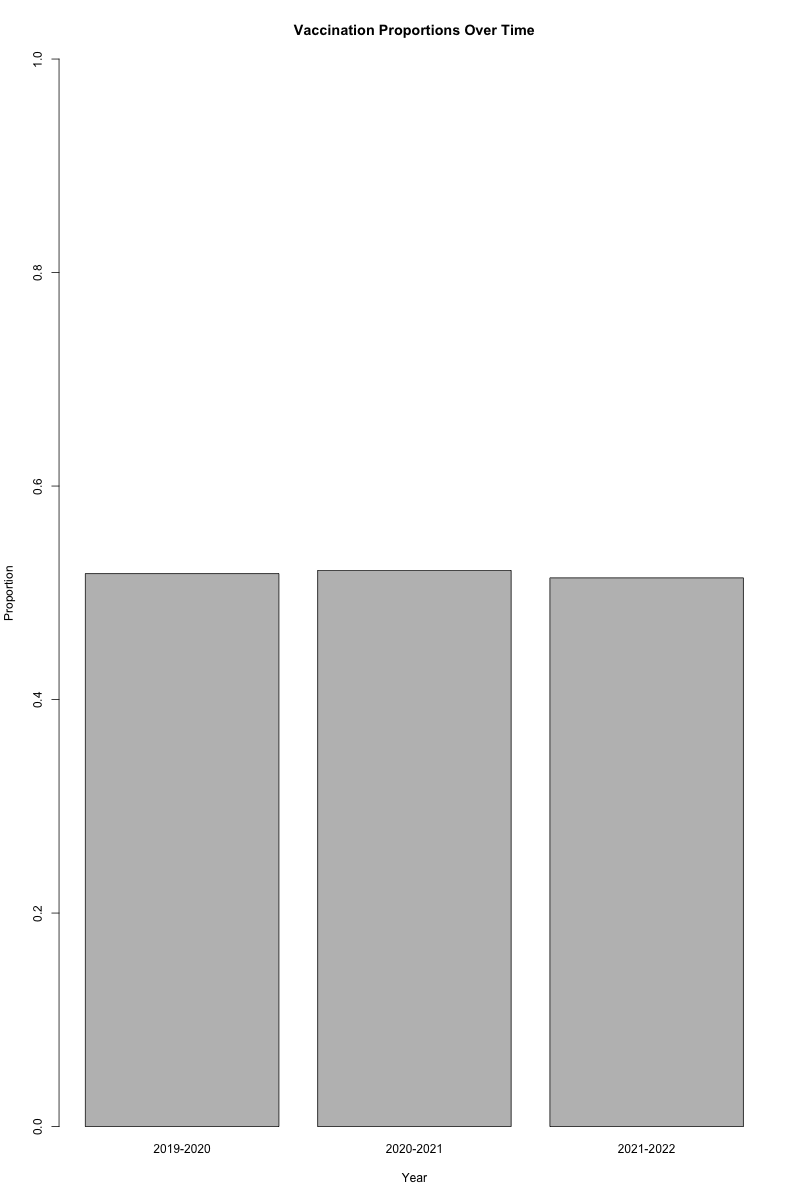
\includegraphics[width= 125mm ,scale=.5]{plot.png}
  \caption{Influenza Vaccination Proportions of Those $\ge 6$ Months Old From 2019-2022.}
  \label{fig:years}
\end{figure}

\begin{figure}[ht!]
  \centering
  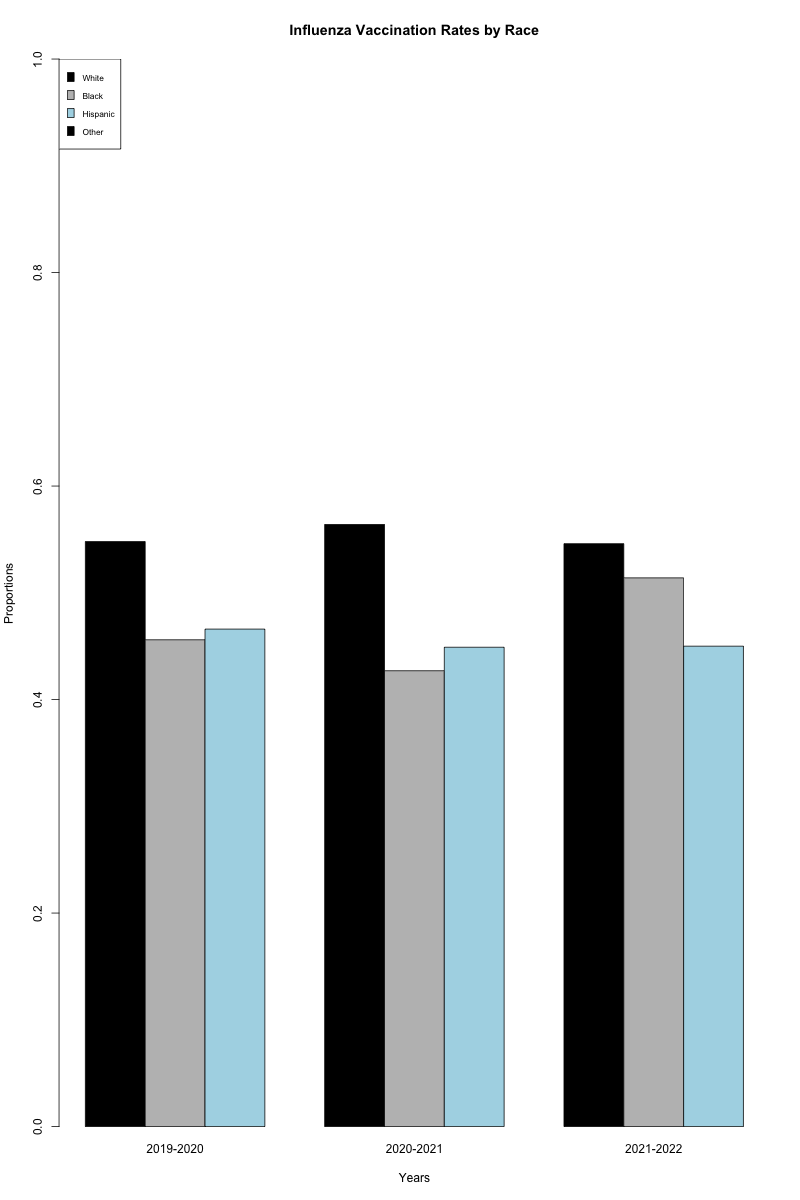
\includegraphics[width= 125mm ,scale=.75]{race.png}
  \caption{Influenza Vaccination Proportions by Race in 2019-2022.}
  \label{fig:race}
\end{figure}

\begin{figure}[ht!]
  \centering
  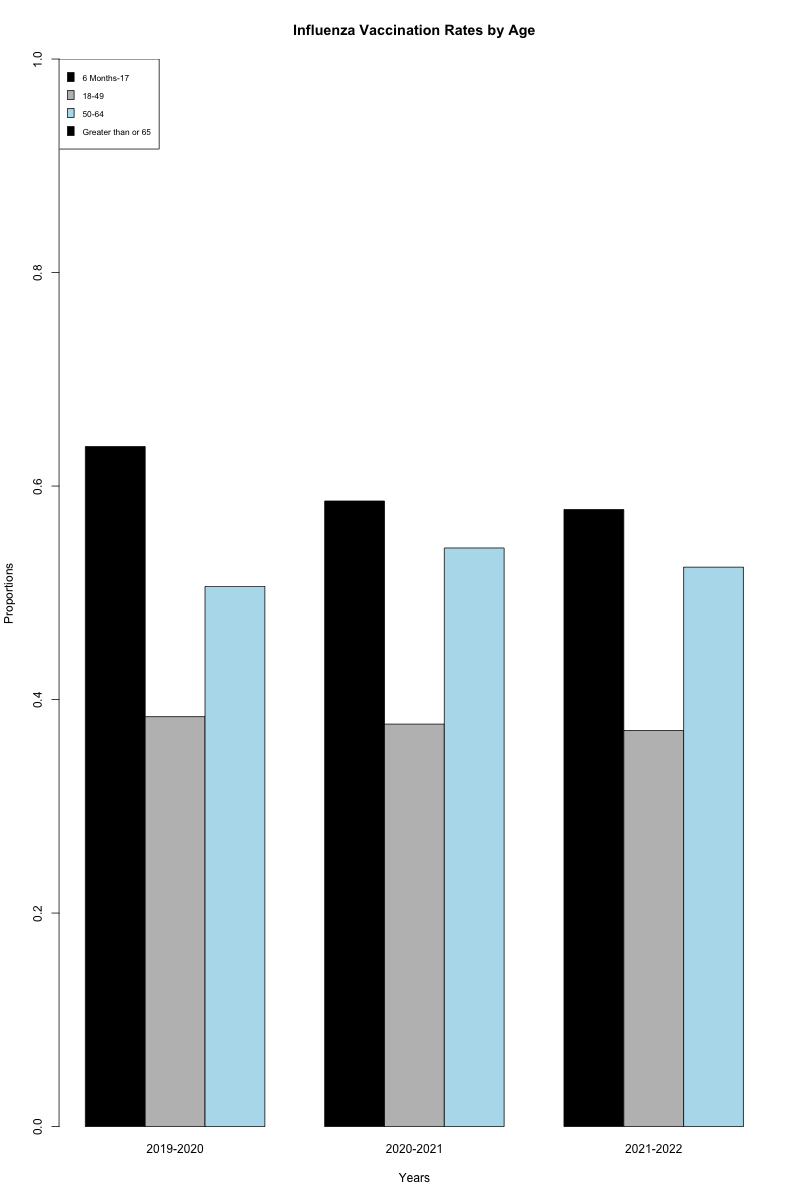
\includegraphics[width= 125mm ,scale=.5]{age.png}
  \caption{Influenza Vaccination Proportions by Age in 2019-2022.}
  \label{fig:age}
\end{figure}

\clearpage
\section{Methods}
\label{sec:Methods}
In order to determine if there was evidence of a significant difference in influenza vaccination proportions, two proportion z tests were conducted using R software. The
hypotheses tested were that there was no significant difference in population proportions verus there was a significant difference. A total of 18 tests were conducted. As stated
earlier, before the Covid-19 pandemic was defined as 2019-2020, during the pandemic was defined as 2020-2021, and after the pandemic was defined as 2021-2022. The following conditions
were assumed to be met in order to use the two proportion z test: the sample size of those interviewed by the CDC for adults in the United States and the age and racial groups chosen
was sufficiently large enough; there were enough successes defined as recieving the influenza vaccine and failures defined as not recieving the influenza vaccine; the groups being compared
at any point in time were independent random samples with observations that were independent from one another. \par
Because R requires the total number of successes to undergo a two proportion z-test, we first needed to calculate how many participants recieved the influenza vaccines within each sample. This was done by simply
taking the total sample size, n, and multiplying it by the proportion reported of those vaccinated. For example, the sample size of adults in the United States vaccinated during 2019-2020 was .518 and
the sample size was 439649, so this number multiplied by .518 yields 227738.182 successes. The tables below summarizes the sample sizes and number of successes calculated. \par
The first test used the proportions of those vaccinated, who were 6 months or older, from 2019-2020, 2020-2021, and 2021-2022. More specfically, the sample proportion
for 2019-2020, .518, was compared to that of 2020-2021, .521. This step was repeated, but for 2020-2021 compared to 2021-2022. The same hypotheses were tested, but this time
controlling for different age groups. More specifically, for age group greater or equal to 6 months to 17 years of age, the sample proportion for 2019-2020 was compared to the sample
proportion for 2020-2021 and the sample proportion corresponding to 2020-2021 was compared to that of 2021-2022. The steps conducted for the age group greater or equal to 6 months to 17 years of 
age were used for the age groups 18-49 years, 50-64 years, and greater than 65 years of age. \par
After the two proportion z tests were conducted for each group, the 95\% confidence intervals and p-values were extracted. An alpha = .05 significance level was used. Thus, if any p-values were less than
.05, they were concluded to be statistically significant and consequently the null hypothesis was rejected.
\begin{table}[ht!]
    \centering
    \caption{Sample Sizes and Number of Successes for 2019-2020}
    \label{tab:table:sizes}
     \begin{tabularx}{.8\textwidth}{X rr}
      \lsptoprule
                &Sample Size & Number of Successes\\
      \midrule
      $\ge 6$ Months & 439649 & 227738.182\\
      $\ge6$ Months-17 years  &   153533  &    97800.521 \\
      18-49 years  &   100057  &    38421.888  \\
      50-64 years &   79794  &    403075.764 \\
      $\ge 65$ years  &   106265  &    74172.97\\
      White & 307406 & 168458.488 \\
      Black & 351757 & 16040.192 \\
      Hispanic & 35632 & 15214.864 \\
      Other & 39992 & 20715.856 \\
      \lspbottomrule
     \end{tabularx}
    \end{table}

\begin{table}[ht!]
    \centering
    \caption{Sample Sizes and Number of Successes for 2020-2021}
    \label{tab:table:sizes2}
     \begin{tabularx}{.8\textwidth}{X rr}
      \lsptoprule
                &Sample Size & Number of Successes\\
      \midrule
      $\ge 6$ Months & 437494 & 227934.374\\
      $\ge6$ Months-17 years  &   145783  &    85428.838 \\
      18-49 years  &   107180  &    40406.86  \\
      50-64 years &   79128  &    54288.7 \\
      $\ge 65$ years  &   105403  &    79263.056\\
      White & 303771 & 171326.844 \\
      Black & 35632 & 15214.864 \\
      Hispanic & 50505 & 22676.745 \\
      Other & 42028 & 21896.588 \\
      \lspbottomrule
     \end{tabularx}
    \end{table}

\begin{table}[ht!]
    \centering
    \caption{Sample Sizes and Number of Successes for 2021-2022}
    \label{tab:table:sizes3}
     \begin{tabularx}{.8\textwidth}{X rr}
      \lsptoprule
                &Sample Size & Number of Successes\\
      \midrule
      $\ge 6$ Months & 449985 & 231292.29\\
      $\ge6$ Months-17 years  &   158146  &    91408.388 \\
      18-49 years  &   105671  &    39203.941  \\
      50-64 years &   77442 &    40579.608 \\
      $\ge 65$ years  &   108726  &    80348.514\\
      White & 309645 & 1690066.17 \\
      Black & 40070 & 17831.15 \\
      Hispanic & 50265 & 22619.25 \\
      Other & 43418 & 22794.45 \\
      \lspbottomrule
     \end{tabularx}
    \end{table}
\clearpage
\section{Results}
\label{sec:Results}
\begin{table}[ht!]
  \centering
  \caption{P-Values and 95\% Confidence Intervals Comparing 2019-2020 to 2020-2021}
  \label{tab:table:results}
   \begin{tabularx}{.8\textwidth}{X rr}
    \lsptoprule
              &P-Value & 95\% Confidence Intervals\\
    \midrule
    $\ge 6$ Months & 0.004926 &  (-0.0050911327, -0.0009088673)\\
    $\ge6$ Months-17 years  &   < 2.2e-16  &    (0.04751027, 0.05448973) \\
    18-49 years  &   0.001038  &    (0.002816745, 0.011183255)  \\
    50-64 years &   < 2.2e-16 &    (-0.1848294, -0.175344) \\
    $\ge 65$ years  &   < 2.2e-16  &  (-0.05779699, -0.05020301) \\
    White & < 2.2e-16 & (-0.01849098, -0.01350902) \\
    Black & < 2.2e-16 & (0.02360678, 0.03439322) \\
    Hispanic & < 2.2e-16 & (0.2125469, 0.2256196) \\
    Other & 0.39 & (-0.009840547, 0.003840547) \\
    \lspbottomrule
   \end{tabularx}
  \end{table}

\begin{table}[ht!]
  \centering
  \caption{P-Values and 95\% Confidence Intervals Comparing 2020-2021 to 2021-2022}
  \label{tab:table:results1}
   \begin{tabularx}{.8\textwidth}{X rr}
    \lsptoprule
              &P-Value & 95\% Confidence Intervals\\
    \midrule
    $\ge 6$ Months & 4.173e-11 &  (0.004920621, 0.009079379)\\
    $\ge6$ Months-17 years  &   7.934e-06  &    (0.004490355, 0.011509645) \\
    18-49 years  &   0.004232  &    ( 0.001888874, 0.010111126)  \\
    50-64 years &   < 2.2e-16 &    (0.1573092, 0.1668650) \\
    $\ge 65$ years  &   < 5.071e-12 &  (0.009310604, 0.016689396) \\
    White & < 2.2e-16 & (0.01551305, 0.02048695) \\
    Black & < 6.218e-07 & (-0.02507495, -0.01092505) \\
    Hispanic & < 0.7497 & (-0.007142669, 0.005142669) \\
    Other & 0.2419 & (-0.010698808, 0.002698808) \\
    \lspbottomrule
   \end{tabularx}
  \end{table}
\clearpage
There is statistically significant evidence in favor of a difference in population proprotions of those with the influenza vaccine before the Covid-19
pandemic compared to those during the the pandemic for all groups except the racial group other. The racial group other had a p-value of .39, which is
greater than alpha = .05, and thus is insignificant. Its 95\% confidence interval was (-0.009840547, 0.003840547), which contains 0, which corresponds to
the results given by the p-value; we failed to reject the null hypothesis. The p-value for those greater than 6 months of age was 0.004926 with a 95\% confidence
interval of (-0.0050911327, -0.0009088673); the p-value for those $\ge 6$ months - 17 years was < 2.2e-16 with a 95\% confidence inerval of (0.04751027, 0.05448973);
the p-value for those 18-49 years of age was 0.001038 with a 95\% confidence interval of (0.002816745, 0.011183255); the p-value for those 50-64 years of age was
< 2.2e-16 with a 95\% confidence interval of (-0.1848294, -0.175344); the p-value for those older than 65 years of age was < 2.2e-16 with a 95\% confidence interval of 
(-0.05779699, -0.05020301); the p-value for the white racial group was < 2.2e-16 with a 95\% confidence interval of (-0.01849098, -0.01350902); the p-value for the black
racial group was < 2.2e-16 with a 95\% confidence interval of (0.02360678, 0.03439322); and the p-value for the hispanic racial group was < 2.2e-16 with a 95\% confidence
interval of (0.2125469, 0.2256196). \par
There is statistically significant evidence in favor of a different in population proportions of those with the influenza vaccine during the Covid-19 pandemic
compared to those after the Covid-19 pandemic except for the hispanic and other racial groups. The hispanic group had a p-value of < 0.7497 with a 95\% confidence interval of 
(-0.007142669, 0.005142669). Because the p-value is greater than alpha = .05 and the 95\% confidence interval contains 0, we failed to reject the null hypothesis and thus, there is no
significant difference in population proportions from 2020-2021 to 2021-2022. The p-value for the other racial group was 0.2419 with a 95\% confidence interval of (-0.010698808, 0.002698808).
Like the results corresponding to the hispanic group, because the p-value is greater than alpha = .05 and the 95\% confidence interval contains 0, we failed to reject the null hypothesis, so there
was no significant difference in population proportions for during the pandemic compared to after. For the groups that had a significant difference in population proportions their results were as followed:
the p-value for those older than 6 months of age was 4.173e-11 with a 95\% confidence interval of (0.004920621, 0.009079379); for those 6 months - 17 years of age, the p-valye was < 2.2e-16  with a 95\%
confidence interval of (0.04751027, 0.05448973); for those 18-49 years of age, the p-value was 0.004232 with a 95\% confidence interval of ( 0.001888874, 0.010111126); for those 50-64 years of age the p-value was
< 2.2e-16 with a 95\% confidence interval of (0.1573092, 0.1668650); for those older than 65 years of age, the p-value was < 5.071e-12 with a 95\% confidence interval (0.009310604, 0.016689396); for the white racial group,
the p-value was < 2.2e-16 with a 95\% confidence interval of (0.01551305, 0.02048695); and for the black racial group, the p-value was < 6.218e-07 with a 95\% confidence interval of (-0.02507495, -0.01092505).
\section{Discussion}
\label{sec:Discussion}
Ultimatley, the goal of this study was to determine how influenza vaccination rates differed before, during, and after the Covid-19 pandemic by comparing sample proportions reported on the CDC website. Past studies have compared
state influenza vaccination rates, but none have explored how the rates changed for various age groups and racial groups. Thus, this study also was able to accomplish this by performing two proportion z-tests on the racial groups
white, black, hispanic, and other and on the age groups $\ge 6$ months, 6 months-17 years, 18-49 years, 50-64 years, and $\ge 65$ years of age. The statistical analysis conducted yieled the following results: comparing before the
pandemic to during, there was statistically significant evidence in favor of a difference in population proportions for all groups except the other racial group. Additionally, when comparing during the pandemic to after, there was
statistically significant evidence in favor of a difference in population proportions for all groups except the other and hispanic groups. This suggests that there may be factors limiting these two racial groups from obtaining the Influenza
vaccine. \par
The limitations of this study were that because the data was collected using a phone interview, results could have been unrepresentative of the population since they surveyed the population using landline phones as well as cellular.
Not everyone has access to either types of phones and there has been a decline in landline telephones due to an increase in price \citep{boland2006emerging}. Additionally, those who answered the survey may have given false statments since
results were not verified using medical records. There was "7.5\% of BRFSS participants who indicated they had been vaccinated but had a missing month and year of vaccination, the month of vaccination was imputed from other survey respondents 
with non-missing month of vaccination matched for week of interview, age group, state of residence, and race/ethnicity using the hot-deck imputation method," so these results could have been inaccurate and unrepresentative of the characteristics of the
participant \citep{cdc_2021}. \par
Additionally, response rates for both surveys were low and were unable to determine whether the paricipants were United States citizens or not. Thus, the results may include data from non-residents. Also, "there may be errors in flu vaccination status due 
to recall error of parents for NIS-Flu and of respondents for BRFSS[...] and errors from incomplete sample frame, nonresponse, and accuracy of reported flu vaccination status might change over time, which could lead to inaccurate assessment of trends in flu 
vaccination coverage \citep{cdc_2021}. In 2020-2021, there was no data collected in the state of Florida, which has a large number of Americans. Similarily in 2021-2022, no data was collected for the state of California for months January to June. The CDC repored that
during 2019-2020, "due to BRFSS interviews not being completed in all months, adult estimates for New Jersey may be subject to differential bias compared with estimates based on the full set of interviews from September 2019-June 2020, and adult estimates for the District of Columbia 
represent vaccination coverage through November rather than through May" \citep{cdc_2021}. In other words, the surveys failed to sample a large proportion of people, which is unrepresentative of the population. \par
Limitations of the statistical analysis include not conducting one-sided 2 sample proportion z-tests to determine whether or not there was a significant increase or decrease in population propotions amongst the groups. Instead, this study only tested the null hypothesis that there was not a
significant difference in population proportions. Additionally, this study only compared proportions prior to the pandemic to during and during to after, but did not take into account comparing proportions before the pandemic to after. Thus, future studies should do so. Future studies should
also continue to explore how vaccination rates compare amongst different racial groups. This study indpendently looked at racial proportions rather than comparing them to each other to determine if any disparities exist. This is essential because it will allow public health researchers to determine
solutions to making sure vaccines are accessible to all racial groups, but especially to those who are at a disadvanatge. 
\clearpage
\bibliographystyle{chicago}
\bibliography{cite}
\end{document} 